\documentclass[../../../main.tex]{subfiles}
\begin{document}

Developing G code to print the developed structures in a non-planar manner involves two tasks. 
First, it is necessary to understand how G-code works and what modifications would need to be made to the code in order to unlock the third axis during printing. 
Next, the structure must be analysed in order to develop the printing paths for the structure, which will be used to write the G-code that allows them to be printed.
This subsection will explain each of these parts.

\subsection{Implementation of non-planar G-code}

G-code (abbreviation for geometric code) is the most widely used computer numerical control (CNC) and 3D printing programming language. 
It is used mainly in computer-aided manufacturing to control automated machine tools, as well as for 3D-printer slicer applications.
G-code instructions are provided to a machine controller that tells the motors where to move, how fast to move, and what path to follow. 
There are many commands available, and depending on the machine being used, some may be added or removed. This manuscript is not intended to be a guide to using G-code, so only the commands that have been used for this project will be introduced\footnote{Readers are encouraged to explore G-code commands on their own. It is always recommended to consult the manuals provided by the firmware developer, in this case \href{https://marlinfw.org/meta/gcode/}{Marlin}.}.

A complete G-code consists of three parts: header, body and footer. 
The header and footer, as their names suggest, are located at the beginning and end of the code, respectively. 
The header contains commands for setting up the machine before manufacturing, such as turning on the motors, heating the extruder or bed, turning on the fans, etc. 
The footer contains commands to end the use of the machine, such as moving the extruder to its home position, cooling the extruder, turning off fans, etc. 
Both blocks are usually the same in all G-codes for a user and/or machine.
The body, on the other hand, is different for each design manufactured. 
It includes all the commands that govern the movement of the head.
The commands used in the header and footer will not be explained as they are considered irrelevant to the purpose of this section. 
In the header, the extruder and bed temperatures are set using the M190 and M109 commands, respectively, and a straight line is printed on one of the edges of the bed to clean the extruder. 
In the footer, the extruder is raised to a relative height of 1 cm, moved to its home position, and the machine is turned off.

In G-code, commands are identified by their code, which consists of a letter and several numbers. 
The letters can be G or M, depending on whether they are commands that control the movement of the tool or, conversely, commands intended to control the machine's status, respectively. 
As for the numbers, they start from 0 to the index of the last available command and are generally simultaneous. 
While it is true that many of these numbers are common to all machines that use G code, the firmware manufacturer ultimately decides on these commands, and it is possible that two machines may have different commands and even numbers. 
In this project, the Marlin v1.1.9 firmware has been used, so the commands included will refer to this firmware.

As the structures used for this project are strut-based, i.e. straight lines, only the G0 and G1 commands will be used. 
Both commands are used to perform linear movements of the head.
A linear move traces a straight line from one point to another, ensuring that the specified axes will arrive simultaneously at the given coordinates (by linear interpolation). 
The speed may change over time following an acceleration curve, according to the acceleration and jerk settings of the given axes.
In fact, both commands are the same and are perfectly interchangeable. 
However, the G0 command is conventionally used for linear movements in which the tool, in this case the extruder, is not used, and the G1 command is used for linear movements in which the tool is used.
They are easy to use and support various positional and tool control parameters. 
As the 3D printer used only has three axes, the parameters that can be used are as follows:
\begin{itemize}
    \item \textbf{X <pos>:} An absolute or relative coordinate on the X axis.
    \item \textbf{Y <pos>:} An absolute or relative coordinate on the Y axis.
    \item \textbf{Z <pos>:} An absolute or relative coordinate on the Z axis.
    \item \textbf{F <rate>:} Set the requested movement rate for this move and any following moves. As with other rate parameters, this value is specified in current units per minute.
    \item \textbf{E <pos>:} An absolute or relative coordinate on the E (extruder) axis. The E axis describes the position of the filament in terms of input to the extruder feeder.
\end{itemize}

It is not necessary to use all parameters every time; if a parameter is not included in a command line, the previous status of that parameter will be used. 
For this purpose, a G1 command is typically included in the header to set the feed rate, F, which will be used throughout the entire print job. 
For example, the command G1 F600 indicates that the print speed will be 600 $mm/min$.
The units conventionally used are millimetres, although they can be modified as desired.
To print in a non-planar manner, simply use the three positional parameters in each G1 command. 
Normally, the Z axis is only used to change layers, and only the X and Y axes are used in each layer. 
However, if all three are used at the same time, it is possible to print in the air. 
For example, the command G1 X0.5 Y0.5 Z1 will print one of the edges of a square pyramid with a base of 1 mm and a height of 1 mm.
The values of the positional parameters will depend on whether an absolute (G90) or relative (G91) positioning system is used. 
In an absolute positioning system, the final position of the extruder is determined with respect to the point considered as the origin. 
In the relative positioning system, the origin is positioned at the extruder's location, and displacements are determined by increments along each axis, as shown in \cref{fig:g90g91}.
In this work, absolute positioning was used.
This also affects the extruder axis, E.

\begin{figure}[!htbp]
    \centering
    

\tikzset{every picture/.style={line width=0.75pt}} %set default line width to 0.75pt        

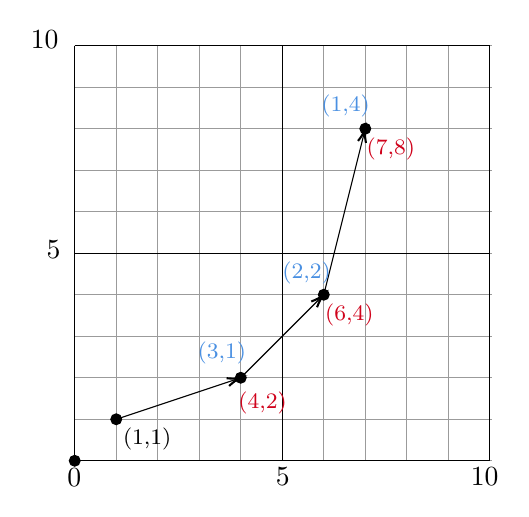
\begin{tikzpicture}[x=0.75pt,y=0.75pt,yscale=-1,xscale=1]
%uncomment if require: \path (0,300); %set diagram left start at 0, and has height of 300

%Shape: Grid [id:dp9135755721036088] 
\draw  [draw opacity=0] (100,66.2) -- (301,66.2) -- (301,266.5) -- (100,266.5) -- cycle ; \draw  [color={rgb, 255:red, 155; green, 155; blue, 155 }  ,draw opacity=1 ] (100,66.2) -- (100,266.5)(120,66.2) -- (120,266.5)(140,66.2) -- (140,266.5)(160,66.2) -- (160,266.5)(180,66.2) -- (180,266.5)(200,66.2) -- (200,266.5)(220,66.2) -- (220,266.5)(240,66.2) -- (240,266.5)(260,66.2) -- (260,266.5)(280,66.2) -- (280,266.5)(300,66.2) -- (300,266.5) ; \draw  [color={rgb, 255:red, 155; green, 155; blue, 155 }  ,draw opacity=1 ] (100,66.2) -- (301,66.2)(100,86.2) -- (301,86.2)(100,106.2) -- (301,106.2)(100,126.2) -- (301,126.2)(100,146.2) -- (301,146.2)(100,166.2) -- (301,166.2)(100,186.2) -- (301,186.2)(100,206.2) -- (301,206.2)(100,226.2) -- (301,226.2)(100,246.2) -- (301,246.2)(100,266.2) -- (301,266.2) ; \draw  [color={rgb, 255:red, 155; green, 155; blue, 155 }  ,draw opacity=1 ]  ;
%Straight Lines [id:da5428588612634048] 
\draw    (100,66.2) -- (100,266.2) ;
%Straight Lines [id:da8039381767256795] 
\draw    (100,66.2) -- (300,66.2) ;
%Straight Lines [id:da697248837047091] 
\draw    (300,266.2) -- (300,66.2) ;
%Straight Lines [id:da48495401334543176] 
\draw    (300,266.2) -- (100,266.2) ;
%Straight Lines [id:da712234155325812] 
\draw    (200,266.2) -- (200,66.2) ;
%Straight Lines [id:da13512977226752643] 
\draw    (100,166.2) -- (300,166.2) ;
%Shape: Circle [id:dp9308085386239336] 
\draw  [fill={rgb, 255:red, 0; green, 0; blue, 0 }  ,fill opacity=1 ] (97.4,266.2) .. controls (97.4,264.76) and (98.56,263.6) .. (100,263.6) .. controls (101.44,263.6) and (102.6,264.76) .. (102.6,266.2) .. controls (102.6,267.64) and (101.44,268.8) .. (100,268.8) .. controls (98.56,268.8) and (97.4,267.64) .. (97.4,266.2) -- cycle ;
%Shape: Circle [id:dp552388250536563] 
\draw  [fill={rgb, 255:red, 0; green, 0; blue, 0 }  ,fill opacity=1 ] (117.4,246.2) .. controls (117.4,244.76) and (118.56,243.6) .. (120,243.6) .. controls (121.44,243.6) and (122.6,244.76) .. (122.6,246.2) .. controls (122.6,247.64) and (121.44,248.8) .. (120,248.8) .. controls (118.56,248.8) and (117.4,247.64) .. (117.4,246.2) -- cycle ;
%Shape: Circle [id:dp8727246455385494] 
\draw  [fill={rgb, 255:red, 0; green, 0; blue, 0 }  ,fill opacity=1 ] (177.4,226.2) .. controls (177.4,224.76) and (178.56,223.6) .. (180,223.6) .. controls (181.44,223.6) and (182.6,224.76) .. (182.6,226.2) .. controls (182.6,227.64) and (181.44,228.8) .. (180,228.8) .. controls (178.56,228.8) and (177.4,227.64) .. (177.4,226.2) -- cycle ;
%Shape: Circle [id:dp2983524848929865] 
\draw  [fill={rgb, 255:red, 0; green, 0; blue, 0 }  ,fill opacity=1 ] (217.4,186.2) .. controls (217.4,184.76) and (218.56,183.6) .. (220,183.6) .. controls (221.44,183.6) and (222.6,184.76) .. (222.6,186.2) .. controls (222.6,187.64) and (221.44,188.8) .. (220,188.8) .. controls (218.56,188.8) and (217.4,187.64) .. (217.4,186.2) -- cycle ;
%Shape: Circle [id:dp25627201303944624] 
\draw  [fill={rgb, 255:red, 0; green, 0; blue, 0 }  ,fill opacity=1 ] (237.4,106.2) .. controls (237.4,104.76) and (238.56,103.6) .. (240,103.6) .. controls (241.44,103.6) and (242.6,104.76) .. (242.6,106.2) .. controls (242.6,107.64) and (241.44,108.8) .. (240,108.8) .. controls (238.56,108.8) and (237.4,107.64) .. (237.4,106.2) -- cycle ;
%Straight Lines [id:da34567719492876536] 
\draw    (120,246.2) -- (178.1,226.83) ;
\draw [shift={(180,226.2)}, rotate = 161.57] [color={rgb, 255:red, 0; green, 0; blue, 0 }  ][line width=0.75]    (6.56,-1.97) .. controls (4.17,-0.84) and (1.99,-0.18) .. (0,0) .. controls (1.99,0.18) and (4.17,0.84) .. (6.56,1.97)   ;
%Straight Lines [id:da106557243100044] 
\draw    (180,226.2) -- (218.59,187.61) ;
\draw [shift={(220,186.2)}, rotate = 135] [color={rgb, 255:red, 0; green, 0; blue, 0 }  ][line width=0.75]    (6.56,-1.97) .. controls (4.17,-0.84) and (1.99,-0.18) .. (0,0) .. controls (1.99,0.18) and (4.17,0.84) .. (6.56,1.97)   ;
%Straight Lines [id:da9122379405009994] 
\draw    (220,186.2) -- (239.51,108.14) ;
\draw [shift={(240,106.2)}, rotate = 104.04] [color={rgb, 255:red, 0; green, 0; blue, 0 }  ][line width=0.75]    (6.56,-1.97) .. controls (4.17,-0.84) and (1.99,-0.18) .. (0,0) .. controls (1.99,0.18) and (4.17,0.84) .. (6.56,1.97)   ;

% Text Node
\draw (95.2,268.8) node [anchor=north west][inner sep=0.75pt]   [align=left] {0};
% Text Node
\draw (195.6,268.2) node [anchor=north west][inner sep=0.75pt]   [align=left] {5};
% Text Node
\draw (289.6,268.2) node [anchor=north west][inner sep=0.75pt]   [align=left] {10};
% Text Node
\draw (85.2,159) node [anchor=north west][inner sep=0.75pt]   [align=left] {5};
% Text Node
\draw (77.6,57.8) node [anchor=north west][inner sep=0.75pt]   [align=left] {10};
% Text Node
\draw (122,249.2) node [anchor=north west][inner sep=0.75pt]  [font=\footnotesize] [align=left] {(1,1)};
% Text Node
\draw (177.6,231.8) node [anchor=north west][inner sep=0.75pt]  [font=\footnotesize,color={rgb, 255:red, 208; green, 2; blue, 27 }  ,opacity=1 ] [align=left] {(4,2)};
% Text Node
\draw (158,207.8) node [anchor=north west][inner sep=0.75pt]  [font=\footnotesize,color={rgb, 255:red, 74; green, 144; blue, 226 }  ,opacity=1 ] [align=left] {(3,1)};
% Text Node
\draw (219.4,189.2) node [anchor=north west][inner sep=0.75pt]  [font=\footnotesize,color={rgb, 255:red, 208; green, 2; blue, 27 }  ,opacity=1 ] [align=left] {(6,4)};
% Text Node
\draw (239.4,109.2) node [anchor=north west][inner sep=0.75pt]  [font=\footnotesize,color={rgb, 255:red, 208; green, 2; blue, 27 }  ,opacity=1 ] [align=left] {(7,8)};
% Text Node
\draw (198.8,169) node [anchor=north west][inner sep=0.75pt]  [font=\footnotesize,color={rgb, 255:red, 74; green, 144; blue, 226 }  ,opacity=1 ] [align=left] {(2,2)};
% Text Node
\draw (217.6,88.6) node [anchor=north west][inner sep=0.75pt]  [font=\footnotesize,color={rgb, 255:red, 74; green, 144; blue, 226 }  ,opacity=1 ] [align=left] {(1,4)};


\end{tikzpicture}

    \caption{Example of the use of the absolute coordinate system, in red, and the relative coordinate system, in blue.}
    \label{fig:g90g91}
\end{figure}

The E parameter corresponds to the amount of filament to be extruded during the movement.
This translates into how much the motors that push the filament towards the extruder have to rotate. 
Generally, to calculate this parameter, it is necessary to calculate the volume of the rectangular prism that is generated when the molten filament exits the extruder and is pressed against the base. 
However, in non-planar printing, this does not happen; instead, the material maintains the same cylindrical shape as it exits. 
Therefore, to calculate this parameter, the volume of the cylinder to be printed must be calculated, see \cref{fig:no_planar}. 

\begin{figure}[!htbp]
    \centering
    

% Gradient Info
  
\tikzset {_oo0z95nez/.code = {\pgfsetadditionalshadetransform{ \pgftransformshift{\pgfpoint{0 bp } { -1.5 bp }  }  \pgftransformrotate{-90 }  \pgftransformscale{2 }  }}}
\pgfdeclarehorizontalshading{_7ukztbkc5}{150bp}{rgb(0bp)=(1,1,1);
rgb(37.5bp)=(1,1,1);
rgb(62.5bp)=(0,0,0);
rgb(100bp)=(0,0,0)}
\tikzset{_fd5st3tr3/.code = {\pgfsetadditionalshadetransform{\pgftransformshift{\pgfpoint{0 bp } { -1.5 bp }  }  \pgftransformrotate{-90 }  \pgftransformscale{2 } }}}
\pgfdeclarehorizontalshading{_j0lyu8nds} {150bp} {color(0bp)=(transparent!0);
color(37.5bp)=(transparent!0);
color(62.5bp)=(transparent!10);
color(100bp)=(transparent!10) } 
\pgfdeclarefading{_l2sq6wasg}{\tikz \fill[shading=_j0lyu8nds,_fd5st3tr3] (0,0) rectangle (50bp,50bp); } 

% Gradient Info
  
\tikzset {_vl71yme9t/.code = {\pgfsetadditionalshadetransform{ \pgftransformshift{\pgfpoint{0 bp } { 0 bp }  }  \pgftransformscale{1 }  }}}
\pgfdeclareradialshading{_vlzwsksb4}{\pgfpoint{0bp}{0bp}}{rgb(0bp)=(1,1,1);
rgb(0bp)=(1,1,1);
rgb(25bp)=(0.96,0.65,0.14);
rgb(400bp)=(0.96,0.65,0.14)}
\tikzset{every picture/.style={line width=0.75pt}} %set default line width to 0.75pt        

\begin{tikzpicture}[x=0.75pt,y=0.75pt,yscale=-1,xscale=1]
%uncomment if require: \path (0,300); %set diagram left start at 0, and has height of 300

%Shape: Path Data [id:dp6219748067424139] 
\path  [shading=_7ukztbkc5,_oo0z95nez,path fading= _l2sq6wasg ,fading transform={xshift=2}] (349.5,135.25) -- (341,135.25) -- (341,56.25) -- (327.5,56.25) -- (327.5,19.25) -- (364.5,19.25) -- (364.5,56.25) -- (349.5,56.25) -- (349.5,135.25) -- cycle ; % for fading 
 \draw   (349.5,135.25) -- (341,135.25) -- (341,56.25) -- (327.5,56.25) -- (327.5,19.25) -- (364.5,19.25) -- (364.5,56.25) -- (349.5,56.25) -- (349.5,135.25) -- cycle ; % for border 

%Shape: Path Data [id:dp1918091195313667] 
\path  [shading=_vlzwsksb4,_vl71yme9t] (182.55,159.77) -- (174.21,159.74) -- (157.81,143.73) -- (199.03,143.86) -- (182.55,159.77) -- cycle (206.25,143.67) -- (150.25,143.67) -- (150.25,119.45) -- (206.25,119.45) -- (206.25,143.67) -- cycle (191.82,63.25) -- (191.82,119.27) -- (164.68,119.27) -- (164.68,63.25) -- (191.82,63.25) -- cycle ; % for fading 
 \draw   (182.55,159.77) -- (174.21,159.74) -- (157.81,143.73) -- (199.03,143.86) -- (182.55,159.77) -- cycle (206.25,143.67) -- (150.25,143.67) -- (150.25,119.45) -- (206.25,119.45) -- (206.25,143.67) -- cycle (191.82,63.25) -- (191.82,119.27) -- (164.68,119.27) -- (164.68,63.25) -- (191.82,63.25) -- cycle ; % for border 

%Shape: Regular Polygon [id:dp2406449410310607] 
\draw   (264.2,162.67) .. controls (264.78,158.17) and (274.8,165.47) .. (295.58,156.21) .. controls (316.35,146.94) and (341.69,135.43) .. (346.21,133.68) .. controls (350.73,131.94) and (349.89,135.66) .. (348.81,136.54) .. controls (347.74,137.42) and (288.95,164.48) .. (280.3,164.69) .. controls (271.66,164.9) and (263.61,167.16) .. (264.2,162.67) -- cycle ;
%Straight Lines [id:da5529504218441703] 
\draw    (177.5,99) -- (222,99.24) ;
\draw [shift={(224,99.25)}, rotate = 180.31] [color={rgb, 255:red, 0; green, 0; blue, 0 }  ][line width=0.75]    (10.93,-3.29) .. controls (6.95,-1.4) and (3.31,-0.3) .. (0,0) .. controls (3.31,0.3) and (6.95,1.4) .. (10.93,3.29)   ;
%Straight Lines [id:da9164514520029656] 
\draw    (345,98) -- (383.17,81.06) ;
\draw [shift={(385,80.25)}, rotate = 156.07] [color={rgb, 255:red, 0; green, 0; blue, 0 }  ][line width=0.75]    (10.93,-3.29) .. controls (6.95,-1.4) and (3.31,-0.3) .. (0,0) .. controls (3.31,0.3) and (6.95,1.4) .. (10.93,3.29)   ;
%Shape: Rectangle [id:dp6644461740443299] 
\draw   (97.37,159.77) -- (182.55,159.77) -- (182.55,164.78) -- (97.37,164.78) -- cycle ;

% Text Node
\draw (196,73) node [anchor=north west][inner sep=0.75pt]  [font=\footnotesize] [align=left] {$\displaystyle \overrightarrow{( x,y)}$};
% Text Node
\draw (357,59) node [anchor=north west][inner sep=0.75pt]  [font=\footnotesize] [align=left] {$\displaystyle \overrightarrow{( x,y,z)}$};


\end{tikzpicture}

    \caption{Illustration of extruded material in planar printing (left) and non-planar printing (right).}
    \label{fig:no_planar}
\end{figure}

Since the diameter of the extruder is fixed, the diameter of the printed cylinder will also be constant. 
This is one of the main drawbacks of this type of printing: to modify the thickness of the cylinders, the diameter of the extruder must be modified. 
As mentioned above, this parameter acts on the motors that push the filament, so the value must be given in relation to the amount of filament that needs to be pushed. 
Therefore, this value is obtained by conserving the mass in the extruder's control volume.
Given the control volume defined in \cref{fig:E}, the amount of material passing through interface $e_1$ must be equal to that passing through interface $e_2$, since the rest of the interfaces are solid.

\begin{figure}[!htbp]
    \centering
    

% Gradient Info
  
\tikzset {_geld2178i/.code = {\pgfsetadditionalshadetransform{ \pgftransformshift{\pgfpoint{0 bp } { 0 bp }  }  \pgftransformrotate{0 }  \pgftransformscale{2 }  }}}
\pgfdeclarehorizontalshading{_8gtsa1tg3}{150bp}{rgb(0bp)=(1,1,1);
rgb(37.5bp)=(1,1,1);
rgb(48.48214285714286bp)=(0.96,0.65,0.14);
rgb(100bp)=(0.96,0.65,0.14)}
\tikzset{every picture/.style={line width=0.75pt}} %set default line width to 0.75pt        

\begin{tikzpicture}[x=0.75pt,y=0.75pt,yscale=-1,xscale=1]
%uncomment if require: \path (0,300); %set diagram left start at 0, and has height of 300

%Shape: Path Data [id:dp9492299757340803] 
\path  [shading=_8gtsa1tg3,_geld2178i] (209.58,169.75) -- (172,169.75) -- (125.15,100.53) -- (125.04,100.53) -- (125.04,51.86) -- (256.43,51.86) -- (256.43,100.53) -- (209.58,169.75) -- cycle ; % for fading 
 \draw   (209.58,169.75) -- (172,169.75) -- (125.15,100.53) -- (125.04,100.53) -- (125.04,51.86) -- (256.43,51.86) -- (256.43,100.53) -- (209.58,169.75) -- cycle ; % for border 

%Shape: Path Data [id:dp15137488085975803] 
\draw  [fill={rgb, 255:red, 74; green, 144; blue, 226 }  ,fill opacity=1 ] (148.35,103.07) -- (148.28,103.07) -- (148.28,72.3) -- (148.33,72.3) -- (148.33,51.86) -- (235.61,51.86) -- (235.61,103.07) -- (204.47,146.83) -- (204.47,197) -- (179.49,197) -- (179.49,146.83) -- (148.35,103.07) -- cycle ;
%Straight Lines [id:da2754383415374976] 
\draw    (150.4,40.6) -- (237.4,41) ;
\draw [shift={(237.4,41)}, rotate = 180.26] [color={rgb, 255:red, 0; green, 0; blue, 0 }  ][line width=0.75]    (0,3.35) -- (0,-3.35)(6.56,-1.97) .. controls (4.17,-0.84) and (1.99,-0.18) .. (0,0) .. controls (1.99,0.18) and (4.17,0.84) .. (6.56,1.97)   ;
\draw [shift={(150.4,40.6)}, rotate = 0.26] [color={rgb, 255:red, 0; green, 0; blue, 0 }  ][line width=0.75]    (0,3.35) -- (0,-3.35)(6.56,-1.97) .. controls (4.17,-0.84) and (1.99,-0.18) .. (0,0) .. controls (1.99,0.18) and (4.17,0.84) .. (6.56,1.97)   ;
%Straight Lines [id:da2165549302677806] 
\draw    (179.6,206.2) -- (205,205.8) ;
\draw [shift={(205,205.8)}, rotate = 179.1] [color={rgb, 255:red, 0; green, 0; blue, 0 }  ][line width=0.75]    (0,3.35) -- (0,-3.35)(6.56,-1.97) .. controls (4.17,-0.84) and (1.99,-0.18) .. (0,0) .. controls (1.99,0.18) and (4.17,0.84) .. (6.56,1.97)   ;
\draw [shift={(179.6,206.2)}, rotate = 359.1] [color={rgb, 255:red, 0; green, 0; blue, 0 }  ][line width=0.75]    (0,3.35) -- (0,-3.35)(6.56,-1.97) .. controls (4.17,-0.84) and (1.99,-0.18) .. (0,0) .. controls (1.99,0.18) and (4.17,0.84) .. (6.56,1.97)   ;
%Shape: Path Data [id:dp5403946800956351] 
\draw  [dash pattern={on 0.84pt off 2.51pt}] (203.62,143) -- (181.11,143) -- (153.06,101.51) -- (153,101.51) -- (153,72.33) -- (231.67,72.33) -- (231.67,101.51) -- (203.62,143) -- cycle ;
%Straight Lines [id:da5188554524250316] 
\draw    (191.67,128.83) -- (191.67,166.17) ;
\draw [shift={(191.67,169.17)}, rotate = 270] [fill={rgb, 255:red, 0; green, 0; blue, 0 }  ][line width=0.08]  [draw opacity=0] (5.36,-2.57) -- (0,0) -- (5.36,2.57) -- cycle    ;
%Straight Lines [id:da22307227495117776] 
\draw    (192,55.5) -- (192,92.83) ;
\draw [shift={(192,95.83)}, rotate = 270] [fill={rgb, 255:red, 0; green, 0; blue, 0 }  ][line width=0.08]  [draw opacity=0] (5.36,-2.57) -- (0,0) -- (5.36,2.57) -- cycle    ;

% Text Node
\draw (185.2,18.4) node [anchor=north west][inner sep=0.75pt]   [align=left] {$\displaystyle D_{f}$};
% Text Node
\draw (184.8,209.8) node [anchor=north west][inner sep=0.75pt]   [align=left] {$\displaystyle d_{e}$};
% Text Node
\draw (197,75) node [anchor=north west][inner sep=0.75pt]   [align=left] {$\displaystyle q_{f}$};
% Text Node
\draw (194.33,118) node [anchor=north west][inner sep=0.75pt]   [align=left] {$\displaystyle q_{e}$};
% Text Node
\draw (156.67,62) node [anchor=north west][inner sep=0.75pt]  [font=\footnotesize] [align=left] {$\displaystyle e_{1}$};
% Text Node
\draw (176,125) node [anchor=north west][inner sep=0.75pt]  [font=\footnotesize] [align=left] {$\displaystyle e_{2}$};
% Text Node
\draw (211.67,57) node [anchor=north west][inner sep=0.75pt]   [align=left] {$\displaystyle V_{c}$};


\end{tikzpicture}

    \caption{Schematic section of a 3D printing extruder. The molten filament is shown in blue and the extruder in orange.}
    \label{fig:E}
\end{figure}

Where $D_f$ is the diameter of the filament and $d_e$ is the diameter of the extruder, the following relationship can be used:
\[
V_f = V_e.
\]
Where
\begin{align*}
V_{f} = E \cdot \frac{\pi D_f^2}{4} \\
V_{e} = \Delta L \cdot \frac{\pi d_e^2}{4}
\end{align*}
Let E be the extrusion parameter sought and $\Delta L$ be the length of the cylinder to extrude. 
If both expressions are equated, the expression for parameter E for non-planar printing can be obtained:

\[
\boxed{E = \Delta L \cdot \frac{d_e^2}{D_f^2}}
\]

This expression is valid regardless of the type of extruder used.
The filament diameter most commonly used in personal printers is 1.75 \textit{mm}, which is the one used in this project. 
As for the extruder, the most common in personal printers is 0.4 \textit{mm}, although various types have been used in this project. 
However, in any case, both parameters are constant, so it is only necessary to know the length of the cylinder to be printed to obtain the E parameter. 
Additionally, this parameter is usually multiplied by another value called flow rate (FR $\in [0,1]$), which is used to modify the value of E if the amount to be extruded needs to be reduced.

\subsection{Strategy for defining printing paths}

Once we have explained how to instruct the printer to print in a non-planar manner, the next objective is to establish the paths that the extruder must follow to print the structure.     

Given that the skeleton of the structure is stored as a graph, graph theory could be used to traverse the graph under certain conditions and thus establish these paths.  
For example, finding the shortest paths that travel through the graph. 
The structure could even be divided into generations of tetrahedra (layers), and the same paths could be searched for between each of the generations. 
The latter method is more viable as it allows the structure to grow gradually, preventing the printer head from colliding with already printed parts if one of the paths found crosses several layers. 
Therefore, the paths should traverse ascending and then descending edges to print the structure continuously. 
There are various graph search algorithms that allow these paths to be found, such as the A* algorithm, Breadth First Search or Depth First Search. 
All of them can include heuristic functions that penalise nodes that prevent the extruder from changing its vertical printing direction. 
Although it is mathematically feasible to find these paths, it is physically unfeasible to use them to print the structure.

It must be kept in mind that the filament inside the extruder is molten, so it behaves like a highly viscous liquid, and once it leaves the extruder, it begins to solidify. Both states are linked by a transition zone just at the extruder outlet, where the polymer will behave viscoelastically, see \cref{fig:no_paths}. The length of this zone will depend on the temperature of the extruder, the ambient temperature and the extrusion speed, and cannot be zero. Determining the length of this zone involves solving a very complex thermodynamic problem, but assuming the filament is a continuous cylindrical body moving at constant speed \( V_f \) in air, a simplified model can be described by equating the heat loss by convection to the internal energy change:

\begin{figure}[!htbp]
    \centering
    

% Gradient Info
  
\tikzset {_ltuftconh/.code = {\pgfsetadditionalshadetransform{ \pgftransformshift{\pgfpoint{0 bp } { -1.5 bp }  }  \pgftransformrotate{-90 }  \pgftransformscale{2 }  }}}
\pgfdeclarehorizontalshading{_116066l99}{150bp}{rgb(0bp)=(1,1,1);
rgb(37.5bp)=(1,1,1);
rgb(62.5bp)=(0,0,0);
rgb(100bp)=(0,0,0)}
\tikzset{_7hyra6oev/.code = {\pgfsetadditionalshadetransform{\pgftransformshift{\pgfpoint{0 bp } { -1.5 bp }  }  \pgftransformrotate{-90 }  \pgftransformscale{2 } }}}
\pgfdeclarehorizontalshading{_tamkewics} {150bp} {color(0bp)=(transparent!0);
color(37.5bp)=(transparent!0);
color(62.5bp)=(transparent!10);
color(100bp)=(transparent!10) } 
\pgfdeclarefading{_2goarmiec}{\tikz \fill[shading=_tamkewics,_7hyra6oev] (0,0) rectangle (50bp,50bp); } 

% Gradient Info
  
\tikzset {_tmoau9aoq/.code = {\pgfsetadditionalshadetransform{ \pgftransformshift{\pgfpoint{0 bp } { 0 bp }  }  \pgftransformrotate{-90 }  \pgftransformscale{2 }  }}}
\pgfdeclarehorizontalshading{_w69zgx8r6}{150bp}{rgb(0bp)=(1,0,0);
rgb(41.607142857142854bp)=(1,0,0);
rgb(49.01785714285714bp)=(1,0,0);
rgb(58.48214285714286bp)=(0.29,0.56,0.89);
rgb(100bp)=(0.29,0.56,0.89)}
\tikzset{every picture/.style={line width=0.75pt}} %set default line width to 0.75pt        

\begin{tikzpicture}[x=0.75pt,y=0.75pt,yscale=-1,xscale=1]
%uncomment if require: \path (0,300); %set diagram left start at 0, and has height of 300

%Shape: Path Data [id:dp4697754887314718] 
\path  [shading=_116066l99,_ltuftconh,path fading= _2goarmiec ,fading transform={xshift=2}] (308.72,191.41) -- (285.13,191.41) -- (285.13,94.42) -- (247.68,94.42) -- (247.68,49) -- (350.33,49) -- (350.33,94.42) -- (308.72,94.42) -- (308.72,191.41) -- cycle ; % for fading 
 \draw   (308.72,191.41) -- (285.13,191.41) -- (285.13,94.42) -- (247.68,94.42) -- (247.68,49) -- (350.33,49) -- (350.33,94.42) -- (308.72,94.42) -- (308.72,191.41) -- cycle ; % for border 

%Shape: Rectangle [id:dp38851785666306216] 
\path  [shading=_w69zgx8r6,_tmoau9aoq] (304.89,294.2) -- (304.89,49) -- (289.37,49) -- (289.37,294.2) -- cycle ; % for fading 
 \draw   (304.89,294.2) -- (304.89,49) -- (289.37,49) -- (289.37,294.2) -- cycle ; % for border 

%Straight Lines [id:da23182528010896997] 
\draw    (271.05,196.32) -- (271.67,254.74) ;
\draw [shift={(271.7,256.74)}, rotate = 269.39] [color={rgb, 255:red, 0; green, 0; blue, 0 }  ][line width=0.75]    (6.56,-1.97) .. controls (4.17,-0.84) and (1.99,-0.18) .. (0,0) .. controls (1.99,0.18) and (4.17,0.84) .. (6.56,1.97)   ;
\draw [shift={(271.03,194.32)}, rotate = 89.39] [color={rgb, 255:red, 0; green, 0; blue, 0 }  ][line width=0.75]    (6.56,-1.97) .. controls (4.17,-0.84) and (1.99,-0.18) .. (0,0) .. controls (1.99,0.18) and (4.17,0.84) .. (6.56,1.97)   ;

% Text Node
\draw (231.51,221.9) node [anchor=north west][inner sep=0.75pt]  [font=\footnotesize] [align=left] {$\displaystyle L_{t}{}_{r}{}_{a}{}_{n}{}_{s}$};


\end{tikzpicture}

    \caption{Schematic illustration of the transition zone of the polymer.}
    \label{fig:no_paths}
\end{figure}

\[
\frac{dQ}{dx} = h_c \cdot A_s \cdot \left( T(x) - T_{\text{air}} \right)
\]

\[
\frac{dQ}{dx} = \rho A c_p V_f \cdot \frac{dT}{dx}
\]

Where:
\begin{itemize}
  \item \( h_c \): convective heat transfer coefficient [W/m\(^2\)K]
  \item \( A_s \): surface area per unit length of the filament (\( \approx 2\pi r \))
  \item \( A \): cross-sectional area of the filament (\( \pi r^2 \))
  \item \( \rho \): density of the material [kg/m\(^3\)]
  \item \( c_p \): specific heat capacity [J/kg·K]
  \item \( V_f \): feed rate [m/s]
  \item \( T(x) \): temperature of the filament at position \( x \)
  \item \( T_{\text{air}} \): ambient air temperature
\end{itemize}

Equating the two expressions:

\[
\rho A c_p V_f \cdot \frac{dT}{dx} = - h_c A_s \cdot \left( T(x) - T_{\text{air}} \right)
\]

Cancelling the geometry (since \( A_s/A = 2/r \)), we get:

\[
\frac{dT}{dx} = -\frac{h_c A_s}{\rho A c_p V_f} (T - T_{\text{air}}) = -\frac{h_c'}{\rho c_p V_f} (T - T_{\text{air}})
\]

Defining the cooling length scale:

\[
\lambda = \frac{\rho c_p V_f}{h_c'}
\]

This leads to the differential equation:

\[
\frac{dT}{dx} = -\frac{1}{\lambda} (T - T_{\text{air}})
\]

This is a standard first-order linear differential equation. Its solution is:

\[
T(x) = T_{\text{air}} + (T_0 - T_{\text{air}}) e^{-x / \lambda}
\]

Where \( T_0 = T_{\text{extrusion}} \) is the initial temperature at \( x = 0 \).
The length of the transition zone \( L_{\text{trans}} \) can be defined as the distance at which the temperature reaches the solidification temperature \( T_{\text{solid}} \). Setting:

\[
T(L_{\text{trans}}) = T_{\text{solid}}
\]

\[
T_{\text{solid}} = T_{\text{air}} + (T_{\text{extrusion}} - T_{\text{air}}) e^{-L_{\text{trans}} / \lambda}
\]

Solving for \( L_{\text{trans}} \):

\[
e^{-L_{\text{trans}} / \lambda} = \frac{T_{\text{solid}} - T_{\text{air}}}{T_{\text{extrusion}} - T_{\text{air}}}
\Rightarrow
L_{\text{trans}} = \lambda \cdot \ln\left( \frac{T_{\text{extrusion}} - T_{\text{air}}}{T_{\text{solid}} - T_{\text{air}}} \right)
\]

Finally, substituting \( \lambda \):

\[
L_{\text{trans}} \simeq \frac{\rho c_p V_f}{h_c'} \cdot \ln\left( \frac{T_{\text{extrusion}} - T_{\text{air}}}{T_{\text{solid}} - T_{\text{air}}} \right)
\]

For example, for PLA, this transition zone can vary between 4 - 10 \textit{mm} according to this simplified model, depending on the printing conditions.

The existence of this transition zone will cause a narrowing in this area during upward movements, as the extruder will exert a dragging force, $F_d$, in the direction of travel and the solid area will exert an equal and opposite adhesive force, $F_a$, see \cref{fig:bending_edges} \textcolor{blue}{(a)}. 
If the adhesive force is not sufficient, the edge will detach from the base. 
During upward movement, this is not very problematic because if the printing speed is slowed down sufficiently, the length of the transition zone can be significantly reduced, and there will be almost no narrowing at the edges. 
The biggest problem arises during downward movements. 
In these cases, a torsional moment, $M_t$, also appears at the base of the ascending edge, causing the material in the transition zone to bend, see \cref{fig:bending_edges} \textcolor{blue}{(b)}. 
As the length of the descending edge increases, the moment becomes greater, and there comes a point where the adhesion force is not sufficient to counteract it, and the edge will collapse, \cref{fig:bending_edges} \textcolor{blue}{(c)}. 
This will happen regardless of the printing speed because $L_{trans}$ cannot be zero, and during the descent, it will be greater because the hot walls of the extruder will be in direct contact with the solid descending edge, causing it to heat up. 
Therefore, it is not possible to print descending edges with only three degrees of freedom in the extruder. 
For this reason, it is physically impossible to use a strategy based on graph search algorithms to create the print paths. The method used can only print ascending edges.

\begin{figure}[!htbp]
    \centering
    

% Gradient Info
  
\tikzset {_az0w2hihs/.code = {\pgfsetadditionalshadetransform{ \pgftransformshift{\pgfpoint{0 bp } { 0 bp }  }  \pgftransformrotate{-270 }  \pgftransformscale{2 }  }}}
\pgfdeclarehorizontalshading{_kzikblmyk}{150bp}{rgb(0bp)=(1,1,1);
rgb(54.82142857142857bp)=(1,1,1);
rgb(62.5bp)=(0.61,0.61,0.61);
rgb(100bp)=(0.61,0.61,0.61)}

% Gradient Info
  
\tikzset {_ki58aoeq5/.code = {\pgfsetadditionalshadetransform{ \pgftransformshift{\pgfpoint{0 bp } { 0 bp }  }  \pgftransformrotate{-270 }  \pgftransformscale{2 }  }}}
\pgfdeclarehorizontalshading{_zqnhzoo5e}{150bp}{rgb(0bp)=(1,1,1);
rgb(54.82142857142857bp)=(1,1,1);
rgb(62.5bp)=(0.61,0.61,0.61);
rgb(100bp)=(0.61,0.61,0.61)}

% Gradient Info
  
\tikzset {_s2ca7cwt4/.code = {\pgfsetadditionalshadetransform{ \pgftransformshift{\pgfpoint{0 bp } { 0 bp }  }  \pgftransformrotate{-270 }  \pgftransformscale{2 }  }}}
\pgfdeclarehorizontalshading{_krjr92v7r}{150bp}{rgb(0bp)=(1,1,1);
rgb(54.82142857142857bp)=(1,1,1);
rgb(62.5bp)=(0.61,0.61,0.61);
rgb(100bp)=(0.61,0.61,0.61)}

% Gradient Info
  
\tikzset {_7zm702kfi/.code = {\pgfsetadditionalshadetransform{ \pgftransformshift{\pgfpoint{0 bp } { 0 bp }  }  \pgftransformrotate{0 }  \pgftransformscale{2 }  }}}
\pgfdeclarehorizontalshading{_sc2zfhq8p}{150bp}{rgb(0bp)=(0.29,0.56,0.89);
rgb(53.66071428571429bp)=(0.29,0.56,0.89);
rgb(62.5bp)=(0.82,0.01,0.11);
rgb(100bp)=(0.82,0.01,0.11)}

% Gradient Info
  
\tikzset {_947g3gh8b/.code = {\pgfsetadditionalshadetransform{ \pgftransformshift{\pgfpoint{0 bp } { -0.5 bp }  }  \pgftransformrotate{-90 }  \pgftransformscale{2 }  }}}
\pgfdeclarehorizontalshading{_mxat92h6q}{150bp}{rgb(0bp)=(1,1,1);
rgb(37.5bp)=(1,1,1);
rgb(62.5bp)=(0,0,0);
rgb(100bp)=(0,0,0)}
\tikzset{_zw40vxy9b/.code = {\pgfsetadditionalshadetransform{\pgftransformshift{\pgfpoint{0 bp } { -0.5 bp }  }  \pgftransformrotate{-90 }  \pgftransformscale{2 } }}}
\pgfdeclarehorizontalshading{_o3fnbd0uv} {150bp} {color(0bp)=(transparent!0);
color(37.5bp)=(transparent!0);
color(62.5bp)=(transparent!10);
color(100bp)=(transparent!10) } 
\pgfdeclarefading{_uc5rmmpr3}{\tikz \fill[shading=_o3fnbd0uv,_zw40vxy9b] (0,0) rectangle (50bp,50bp); } 

% Gradient Info
  
\tikzset {_oj9djzokq/.code = {\pgfsetadditionalshadetransform{ \pgftransformshift{\pgfpoint{0 bp } { 0 bp }  }  \pgftransformrotate{0 }  \pgftransformscale{2 }  }}}
\pgfdeclarehorizontalshading{_21zbm29sn}{150bp}{rgb(0bp)=(0.29,0.56,0.89);
rgb(52.85714285714286bp)=(0.29,0.56,0.89);
rgb(62.5bp)=(0.82,0.01,0.11);
rgb(100bp)=(0.82,0.01,0.11)}

% Gradient Info
  
\tikzset {_tvqijb5p1/.code = {\pgfsetadditionalshadetransform{ \pgftransformshift{\pgfpoint{0 bp } { -0.5 bp }  }  \pgftransformrotate{-90 }  \pgftransformscale{2 }  }}}
\pgfdeclarehorizontalshading{_8o8j9rz05}{150bp}{rgb(0bp)=(1,1,1);
rgb(37.5bp)=(1,1,1);
rgb(62.5bp)=(0,0,0);
rgb(100bp)=(0,0,0)}
\tikzset{_p06f5zkm0/.code = {\pgfsetadditionalshadetransform{\pgftransformshift{\pgfpoint{0 bp } { -0.5 bp }  }  \pgftransformrotate{-90 }  \pgftransformscale{2 } }}}
\pgfdeclarehorizontalshading{_wcrn90ura} {150bp} {color(0bp)=(transparent!0);
color(37.5bp)=(transparent!0);
color(62.5bp)=(transparent!10);
color(100bp)=(transparent!10) } 
\pgfdeclarefading{_y8qb6ci5m}{\tikz \fill[shading=_wcrn90ura,_p06f5zkm0] (0,0) rectangle (50bp,50bp); } 

% Gradient Info
  
\tikzset {_0coqb587w/.code = {\pgfsetadditionalshadetransform{ \pgftransformshift{\pgfpoint{0 bp } { 0 bp }  }  \pgftransformrotate{0 }  \pgftransformscale{2 }  }}}
\pgfdeclarehorizontalshading{_5rnivun9u}{150bp}{rgb(0bp)=(0.29,0.56,0.89);
rgb(56.51785714285714bp)=(0.29,0.56,0.89);
rgb(62.5bp)=(0.82,0.01,0.11);
rgb(100bp)=(0.82,0.01,0.11)}

% Gradient Info
  
\tikzset {_863t0pjv8/.code = {\pgfsetadditionalshadetransform{ \pgftransformshift{\pgfpoint{0 bp } { -0.5 bp }  }  \pgftransformrotate{-90 }  \pgftransformscale{2 }  }}}
\pgfdeclarehorizontalshading{_9vc02l939}{150bp}{rgb(0bp)=(1,1,1);
rgb(37.5bp)=(1,1,1);
rgb(62.5bp)=(0,0,0);
rgb(100bp)=(0,0,0)}
\tikzset{_db30gnpfg/.code = {\pgfsetadditionalshadetransform{\pgftransformshift{\pgfpoint{0 bp } { -0.5 bp }  }  \pgftransformrotate{-90 }  \pgftransformscale{2 } }}}
\pgfdeclarehorizontalshading{_np1wbih0r} {150bp} {color(0bp)=(transparent!0);
color(37.5bp)=(transparent!0);
color(62.5bp)=(transparent!10);
color(100bp)=(transparent!10) } 
\pgfdeclarefading{_0q079ch7h}{\tikz \fill[shading=_np1wbih0r,_db30gnpfg] (0,0) rectangle (50bp,50bp); } 
\tikzset{every picture/.style={line width=0.75pt}} %set default line width to 0.75pt        

\begin{tikzpicture}[x=0.75pt,y=0.75pt,yscale=-1,xscale=1]
%uncomment if require: \path (0,300); %set diagram left start at 0, and has height of 300

%Shape: Square [id:dp8482883529416775] 
\draw  [draw opacity=0][shading=_kzikblmyk,_az0w2hihs] (366.67,189.33) -- (409.67,189.33) -- (409.67,232.33) -- (366.67,232.33) -- cycle ;
%Shape: Square [id:dp07525304880654671] 
\draw  [draw opacity=0][shading=_zqnhzoo5e,_ki58aoeq5] (223.33,188.67) -- (266.33,188.67) -- (266.33,231.67) -- (223.33,231.67) -- cycle ;
%Shape: Square [id:dp3833070704623305] 
\draw  [draw opacity=0][shading=_krjr92v7r,_s2ca7cwt4] (95,189.33) -- (138,189.33) -- (138,232.33) -- (95,232.33) -- cycle ;
%Shape: Path Data [id:dp1823169117970066] 
\path  [shading=_sc2zfhq8p,_7zm702kfi] (171.65,150.76) .. controls (171.95,151.2) and (171.85,151.8) .. (171.42,152.11) -- (120.9,188.35) .. controls (120.72,188.66) and (120.38,188.87) .. (119.99,188.87) -- (111.97,188.87) .. controls (111.38,188.87) and (110.9,188.38) .. (110.9,187.78) -- (110.9,184.52) .. controls (110.9,183.92) and (111.38,183.43) .. (111.97,183.43) -- (119.53,183.43) -- (165.44,150.49) -- (165.44,134.2) -- (171.13,134.2) -- (171.13,150.01) -- (171.65,150.76) -- cycle ; % for fading 
 \draw   (171.65,150.76) .. controls (171.95,151.2) and (171.85,151.8) .. (171.42,152.11) -- (120.9,188.35) .. controls (120.72,188.66) and (120.38,188.87) .. (119.99,188.87) -- (111.97,188.87) .. controls (111.38,188.87) and (110.9,188.38) .. (110.9,187.78) -- (110.9,184.52) .. controls (110.9,183.92) and (111.38,183.43) .. (111.97,183.43) -- (119.53,183.43) -- (165.44,150.49) -- (165.44,134.2) -- (171.13,134.2) -- (171.13,150.01) -- (171.65,150.76) -- cycle ; % for border 

%Shape: Path Data [id:dp7664852483691857] 
\path  [shading=_mxat92h6q,_947g3gh8b,path fading= _uc5rmmpr3 ,fading transform={xshift=2}] (172.5,150.75) -- (164,150.75) -- (164,71.75) -- (150.5,71.75) -- (150.5,34.75) -- (187.5,34.75) -- (187.5,71.75) -- (172.5,71.75) -- (172.5,150.75) -- cycle ; % for fading 
 \draw   (172.5,150.75) -- (164,150.75) -- (164,71.75) -- (150.5,71.75) -- (150.5,34.75) -- (187.5,34.75) -- (187.5,71.75) -- (172.5,71.75) -- (172.5,150.75) -- cycle ; % for border 

%Straight Lines [id:da8372784781387078] 
\draw    (168.86,143.14) -- (195.4,123.34) ;
\draw [shift={(197,122.14)}, rotate = 143.27] [color={rgb, 255:red, 0; green, 0; blue, 0 }  ][line width=0.75]    (6.56,-1.97) .. controls (4.17,-0.84) and (1.99,-0.18) .. (0,0) .. controls (1.99,0.18) and (4.17,0.84) .. (6.56,1.97)   ;
\draw [shift={(168.86,143.14)}, rotate = 323.27] [color={rgb, 255:red, 0; green, 0; blue, 0 }  ][fill={rgb, 255:red, 0; green, 0; blue, 0 }  ][line width=0.75]      (0, 0) circle [x radius= 2.01, y radius= 2.01]   ;
%Straight Lines [id:da5883622865301662] 
\draw    (115.71,186.57) -- (85.18,208.96) ;
\draw [shift={(83.57,210.14)}, rotate = 323.75] [color={rgb, 255:red, 0; green, 0; blue, 0 }  ][line width=0.75]    (6.56,-1.97) .. controls (4.17,-0.84) and (1.99,-0.18) .. (0,0) .. controls (1.99,0.18) and (4.17,0.84) .. (6.56,1.97)   ;
\draw [shift={(115.71,186.57)}, rotate = 143.75] [color={rgb, 255:red, 0; green, 0; blue, 0 }  ][fill={rgb, 255:red, 0; green, 0; blue, 0 }  ][line width=0.75]      (0, 0) circle [x radius= 2.01, y radius= 2.01]   ;
%Straight Lines [id:da9559015453503384] 
\draw    (115.71,186.57) -- (115.52,169.75) ;
\draw [shift={(115.5,167.75)}, rotate = 89.35] [color={rgb, 255:red, 0; green, 0; blue, 0 }  ][line width=0.75]    (6.56,-1.97) .. controls (4.17,-0.84) and (1.99,-0.18) .. (0,0) .. controls (1.99,0.18) and (4.17,0.84) .. (6.56,1.97)   ;
\draw [shift={(115.71,186.57)}, rotate = 269.35] [color={rgb, 255:red, 0; green, 0; blue, 0 }  ][fill={rgb, 255:red, 0; green, 0; blue, 0 }  ][line width=0.75]      (0, 0) circle [x radius= 2.01, y radius= 2.01]   ;
%Straight Lines [id:da8008989184780188] 
\draw    (146.71,167.57) -- (146.52,188.75) ;
\draw [shift={(146.5,190.75)}, rotate = 270.53] [color={rgb, 255:red, 0; green, 0; blue, 0 }  ][line width=0.75]    (6.56,-1.97) .. controls (4.17,-0.84) and (1.99,-0.18) .. (0,0) .. controls (1.99,0.18) and (4.17,0.84) .. (6.56,1.97)   ;
\draw [shift={(146.71,167.57)}, rotate = 90.53] [color={rgb, 255:red, 0; green, 0; blue, 0 }  ][fill={rgb, 255:red, 0; green, 0; blue, 0 }  ][line width=0.75]      (0, 0) circle [x radius= 2.01, y radius= 2.01]   ;
%Shape: Path Data [id:dp9292649336162639] 
\path  [shading=_21zbm29sn,_oj9djzokq] (241.44,183.13) -- (250.08,183.13) -- (302.2,136.68) .. controls (302.34,136.56) and (302.5,136.48) .. (302.66,136.43) .. controls (302.72,136.34) and (302.79,136.26) .. (302.87,136.18) -- (305.37,133.91) .. controls (305.83,133.49) and (306.54,133.53) .. (306.96,133.99) -- (316.05,143.99) -- (316.05,132.53) .. controls (316.05,131.9) and (316.56,131.4) .. (317.18,131.4) -- (320.55,131.4) .. controls (321.18,131.4) and (321.68,131.9) .. (321.68,132.53) -- (321.68,152.23) .. controls (321.68,152.85) and (321.18,153.36) .. (320.55,153.36) -- (317.18,153.36) .. controls (316.6,153.36) and (316.12,152.92) .. (316.06,152.36) .. controls (316.06,152.36) and (316.05,152.36) .. (316.05,152.35) -- (305.77,141.04) -- (252.9,188.15) .. controls (252.57,188.45) and (252.11,188.51) .. (251.73,188.36) .. controls (251.72,188.36) and (251.71,188.36) .. (251.7,188.36) -- (241.44,188.36) .. controls (240.86,188.36) and (240.39,187.89) .. (240.39,187.31) -- (240.39,184.17) .. controls (240.39,183.59) and (240.86,183.13) .. (241.44,183.13) -- cycle ; % for fading 
 \draw   (241.44,183.13) -- (250.08,183.13) -- (302.2,136.68) .. controls (302.34,136.56) and (302.5,136.48) .. (302.66,136.43) .. controls (302.72,136.34) and (302.79,136.26) .. (302.87,136.18) -- (305.37,133.91) .. controls (305.83,133.49) and (306.54,133.53) .. (306.96,133.99) -- (316.05,143.99) -- (316.05,132.53) .. controls (316.05,131.9) and (316.56,131.4) .. (317.18,131.4) -- (320.55,131.4) .. controls (321.18,131.4) and (321.68,131.9) .. (321.68,132.53) -- (321.68,152.23) .. controls (321.68,152.85) and (321.18,153.36) .. (320.55,153.36) -- (317.18,153.36) .. controls (316.6,153.36) and (316.12,152.92) .. (316.06,152.36) .. controls (316.06,152.36) and (316.05,152.36) .. (316.05,152.35) -- (305.77,141.04) -- (252.9,188.15) .. controls (252.57,188.45) and (252.11,188.51) .. (251.73,188.36) .. controls (251.72,188.36) and (251.71,188.36) .. (251.7,188.36) -- (241.44,188.36) .. controls (240.86,188.36) and (240.39,187.89) .. (240.39,187.31) -- (240.39,184.17) .. controls (240.39,183.59) and (240.86,183.13) .. (241.44,183.13) -- cycle ; % for border 

%Shape: Path Data [id:dp640912868425004] 
\path  [shading=_8o8j9rz05,_tvqijb5p1,path fading= _y8qb6ci5m ,fading transform={xshift=2}] (323.2,148.67) -- (314.7,148.67) -- (314.7,69.67) -- (301.2,69.67) -- (301.2,32.67) -- (338.2,32.67) -- (338.2,69.67) -- (323.2,69.67) -- (323.2,148.67) -- cycle ; % for fading 
 \draw   (323.2,148.67) -- (314.7,148.67) -- (314.7,69.67) -- (301.2,69.67) -- (301.2,32.67) -- (338.2,32.67) -- (338.2,69.67) -- (323.2,69.67) -- (323.2,148.67) -- cycle ; % for border 

%Straight Lines [id:da4735344307781033] 
\draw    (244.38,185.57) -- (227.51,194.68) -- (211.09,203.55) ;
\draw [shift={(209.33,204.5)}, rotate = 331.63] [color={rgb, 255:red, 0; green, 0; blue, 0 }  ][line width=0.75]    (6.56,-1.97) .. controls (4.17,-0.84) and (1.99,-0.18) .. (0,0) .. controls (1.99,0.18) and (4.17,0.84) .. (6.56,1.97)   ;
\draw [shift={(244.38,185.57)}, rotate = 151.63] [color={rgb, 255:red, 0; green, 0; blue, 0 }  ][fill={rgb, 255:red, 0; green, 0; blue, 0 }  ][line width=0.75]      (0, 0) circle [x radius= 2.01, y radius= 2.01]   ;
%Straight Lines [id:da8646577096120663] 
\draw    (318.51,150.44) -- (327.68,160.41) -- (343.45,177.56) ;
\draw [shift={(344.8,179.03)}, rotate = 227.41] [color={rgb, 255:red, 0; green, 0; blue, 0 }  ][line width=0.75]    (6.56,-1.97) .. controls (4.17,-0.84) and (1.99,-0.18) .. (0,0) .. controls (1.99,0.18) and (4.17,0.84) .. (6.56,1.97)   ;
\draw [shift={(318.51,150.44)}, rotate = 47.41] [color={rgb, 255:red, 0; green, 0; blue, 0 }  ][fill={rgb, 255:red, 0; green, 0; blue, 0 }  ][line width=0.75]      (0, 0) circle [x radius= 2.01, y radius= 2.01]   ;
%Shape: Arc [id:dp05193043475644299] 
\draw  [draw opacity=0] (253.64,202.05) .. controls (251.83,202.66) and (249.87,203) .. (247.83,203) .. controls (238.17,203) and (230.33,195.43) .. (230.33,186.08) .. controls (230.33,176.74) and (238.17,169.17) .. (247.83,169.17) .. controls (249.87,169.17) and (251.83,169.5) .. (253.64,170.12) -- (247.83,186.08) -- cycle ; \draw    (253.64,202.05) .. controls (251.83,202.66) and (249.87,203) .. (247.83,203) .. controls (238.17,203) and (230.33,195.43) .. (230.33,186.08) .. controls (230.33,176.74) and (238.17,169.17) .. (247.83,169.17) .. controls (248.83,169.17) and (249.81,169.25) .. (250.76,169.4) ; \draw [shift={(253.64,170.12)}, rotate = 186.14] [fill={rgb, 255:red, 0; green, 0; blue, 0 }  ][line width=0.08]  [draw opacity=0] (5.36,-2.57) -- (0,0) -- (5.36,2.57) -- cycle    ; 
%Shape: Path Data [id:dp083988650529362] 
\path  [shading=_5rnivun9u,_0coqb587w] (385.22,183.51) -- (393.45,183.51) .. controls (393.56,183.28) and (393.74,183.09) .. (393.97,182.95) -- (453.28,149.81) .. controls (453.59,149.63) and (453.95,149.6) .. (454.26,149.7) .. controls (460.2,149.16) and (466.69,150.06) .. (473.03,152.6) .. controls (475.95,153.76) and (478.64,155.2) .. (481.08,156.84) -- (481.08,145.87) .. controls (481.08,145.17) and (481.65,144.6) .. (482.35,144.6) -- (486.15,144.6) .. controls (486.85,144.6) and (487.42,145.17) .. (487.42,145.87) -- (487.42,163.6) .. controls (487.42,164.3) and (486.85,164.86) .. (486.15,164.86) -- (482.35,164.86) .. controls (482.1,164.86) and (481.86,164.79) .. (481.66,164.66) -- (481.35,164.86) .. controls (478.42,162.25) and (474.83,160) .. (470.73,158.36) .. controls (465.56,156.29) and (460.31,155.48) .. (455.53,155.78) -- (455.52,155.74) -- (397.03,188.43) .. controls (396.74,188.59) and (396.42,188.62) .. (396.12,188.55) .. controls (395.93,188.76) and (395.65,188.89) .. (395.34,188.89) -- (385.22,188.89) .. controls (384.63,188.89) and (384.15,188.4) .. (384.15,187.81) -- (384.15,184.58) .. controls (384.15,183.99) and (384.63,183.51) .. (385.22,183.51) -- cycle ; % for fading 
 \draw   (385.22,183.51) -- (393.45,183.51) .. controls (393.56,183.28) and (393.74,183.09) .. (393.97,182.95) -- (453.28,149.81) .. controls (453.59,149.63) and (453.95,149.6) .. (454.26,149.7) .. controls (460.2,149.16) and (466.69,150.06) .. (473.03,152.6) .. controls (475.95,153.76) and (478.64,155.2) .. (481.08,156.84) -- (481.08,145.87) .. controls (481.08,145.17) and (481.65,144.6) .. (482.35,144.6) -- (486.15,144.6) .. controls (486.85,144.6) and (487.42,145.17) .. (487.42,145.87) -- (487.42,163.6) .. controls (487.42,164.3) and (486.85,164.86) .. (486.15,164.86) -- (482.35,164.86) .. controls (482.1,164.86) and (481.86,164.79) .. (481.66,164.66) -- (481.35,164.86) .. controls (478.42,162.25) and (474.83,160) .. (470.73,158.36) .. controls (465.56,156.29) and (460.31,155.48) .. (455.53,155.78) -- (455.52,155.74) -- (397.03,188.43) .. controls (396.74,188.59) and (396.42,188.62) .. (396.12,188.55) .. controls (395.93,188.76) and (395.65,188.89) .. (395.34,188.89) -- (385.22,188.89) .. controls (384.63,188.89) and (384.15,188.4) .. (384.15,187.81) -- (384.15,184.58) .. controls (384.15,183.99) and (384.63,183.51) .. (385.22,183.51) -- cycle ; % for border 

%Shape: Path Data [id:dp4888310079490593] 
\path  [shading=_9vc02l939,_863t0pjv8,path fading= _0q079ch7h ,fading transform={xshift=2}] (488.5,161.47) -- (480,161.47) -- (480,82.47) -- (466.5,82.47) -- (466.5,45.47) -- (503.5,45.47) -- (503.5,82.47) -- (488.5,82.47) -- (488.5,161.47) -- cycle ; % for fading 
 \draw   (488.5,161.47) -- (480,161.47) -- (480,82.47) -- (466.5,82.47) -- (466.5,45.47) -- (503.5,45.47) -- (503.5,82.47) -- (488.5,82.47) -- (488.5,161.47) -- cycle ; % for border 

%Straight Lines [id:da7299773302791036] 
\draw    (389.58,186.37) -- (372.71,195.48) -- (356.29,204.35) ;
\draw [shift={(354.53,205.3)}, rotate = 331.63] [color={rgb, 255:red, 0; green, 0; blue, 0 }  ][line width=0.75]    (6.56,-1.97) .. controls (4.17,-0.84) and (1.99,-0.18) .. (0,0) .. controls (1.99,0.18) and (4.17,0.84) .. (6.56,1.97)   ;
\draw [shift={(389.58,186.37)}, rotate = 151.63] [color={rgb, 255:red, 0; green, 0; blue, 0 }  ][fill={rgb, 255:red, 0; green, 0; blue, 0 }  ][line width=0.75]      (0, 0) circle [x radius= 2.01, y radius= 2.01]   ;
%Shape: Arc [id:dp5816487923294394] 
\draw  [draw opacity=0] (398.84,202.85) .. controls (397.03,203.46) and (395.07,203.8) .. (393.03,203.8) .. controls (383.37,203.8) and (375.53,196.23) .. (375.53,186.88) .. controls (375.53,177.54) and (383.37,169.97) .. (393.03,169.97) .. controls (395.07,169.97) and (397.03,170.3) .. (398.84,170.92) -- (393.03,186.88) -- cycle ; \draw    (398.84,202.85) .. controls (397.03,203.46) and (395.07,203.8) .. (393.03,203.8) .. controls (383.37,203.8) and (375.53,196.23) .. (375.53,186.88) .. controls (375.53,177.54) and (383.37,169.97) .. (393.03,169.97) .. controls (394.03,169.97) and (395.01,170.05) .. (395.96,170.2) ; \draw [shift={(398.84,170.92)}, rotate = 186.14] [fill={rgb, 255:red, 0; green, 0; blue, 0 }  ][line width=0.08]  [draw opacity=0] (5.36,-2.57) -- (0,0) -- (5.36,2.57) -- cycle    ; 
%Straight Lines [id:da3777206426102483] 
\draw    (484.51,160.84) -- (515.39,183.42) ;
\draw [shift={(517,184.6)}, rotate = 216.18] [color={rgb, 255:red, 0; green, 0; blue, 0 }  ][line width=0.75]    (6.56,-1.97) .. controls (4.17,-0.84) and (1.99,-0.18) .. (0,0) .. controls (1.99,0.18) and (4.17,0.84) .. (6.56,1.97)   ;
\draw [shift={(484.51,160.84)}, rotate = 36.18] [color={rgb, 255:red, 0; green, 0; blue, 0 }  ][fill={rgb, 255:red, 0; green, 0; blue, 0 }  ][line width=0.75]      (0, 0) circle [x radius= 2.01, y radius= 2.01]   ;

% Text Node
\draw (185.43,133.57) node [anchor=north west][inner sep=0.75pt]  [font=\small] [align=left] {$\displaystyle \overrightarrow{F_{d}}$};
% Text Node
\draw (97.43,199.29) node [anchor=north west][inner sep=0.75pt]  [font=\small] [align=left] {$\displaystyle \overrightarrow{F_{a}}$};
% Text Node
\draw (117.43,143.79) node [anchor=north west][inner sep=0.75pt]  [font=\small] [align=left] {$\displaystyle \overrightarrow{F_{N}}$};
% Text Node
\draw (152.43,179.29) node [anchor=north west][inner sep=0.75pt]  [font=\small] [align=left] {$\displaystyle \overrightarrow{F_{g}}$};
% Text Node
\draw (214.76,199.95) node [anchor=north west][inner sep=0.75pt]  [font=\small] [align=left] {$\displaystyle \overrightarrow{F_{a}}$};
% Text Node
\draw (334.43,140.57) node [anchor=north west][inner sep=0.75pt]  [font=\small] [align=left] {$\displaystyle \overrightarrow{F_{d}}$};
% Text Node
\draw (231.76,144.29) node [anchor=north west][inner sep=0.75pt]  [font=\small] [align=left] {$\displaystyle \overrightarrow{M_{T}}$};
% Text Node
\draw (359.96,200.75) node [anchor=north west][inner sep=0.75pt]  [font=\small] [align=left] {$\displaystyle \overrightarrow{F_{a}}$};
% Text Node
\draw (376.96,145.09) node [anchor=north west][inner sep=0.75pt]  [font=\small] [align=left] {$\displaystyle \overrightarrow{M_{T}}$};
% Text Node
\draw (500.83,149.37) node [anchor=north west][inner sep=0.75pt]  [font=\small] [align=left] {$\displaystyle \overrightarrow{F_{d}}$};
% Text Node
\draw (152.67,231.67) node [anchor=north west][inner sep=0.75pt]   [align=left] {A)};
% Text Node
\draw (303.33,232.33) node [anchor=north west][inner sep=0.75pt]   [align=left] {B)};
% Text Node
\draw (476.67,229.67) node [anchor=north west][inner sep=0.75pt]   [align=left] {C)};


\end{tikzpicture}

    \caption{Schematic illustration of the evolution of the state of an edge printed upwards and then downwards.}
    \label{fig:bending_edges}
\end{figure}


Therefore, it was decided to divide the structure by generations and print each of the tetrahedra that comprises them individually. 
This way, each edge is printed in ascending order. 
As the layers are composed of tetrahedra of varying shapes and heights, a method must be devised that enables them to be printed without collapsing onto previously printed parts due to collisions with the print head. 
To do this, the tetrahedra are sorted according to their height and printed from the lowest to the highest. 
This may not guarantee that the print head will not collide with the printed parts, but it does guarantee that if there are any collisions, they will be as few as possible. 
For example, in \cref{fig:printing_tets} \textcolor{blue}{(a)}, printing the triangle on the right first could cause the print head to collide with that pyramid three times, once for each edge printed after the first. 
However, if the one on the left is printed first, it could only collide once; once the small triangle is printed, it cannot collide with it again. 
The probability of collision will depend on the length of the tetrahedra and the length of the extruder. 
For this reason, the longer the extruder, the better. 
It is also necessary to clarify the printing order of each of the edges of a tetrahedron. 
As there may be tetrahedra with internal edges, it is always better to print those edges first. 
Otherwise, the head would collide with the outer edges that have already been printed. 
Therefore, it was decided that the order of the edges would depend on the distance from the base of each edge to the projection of the tetrahedron's vertex on the base, see \cref{fig:printing_tets} \textcolor{blue}{(b)}.

\begin{figure}[!htbp]
    \centering
    

\tikzset{every picture/.style={line width=0.75pt}} %set default line width to 0.75pt        

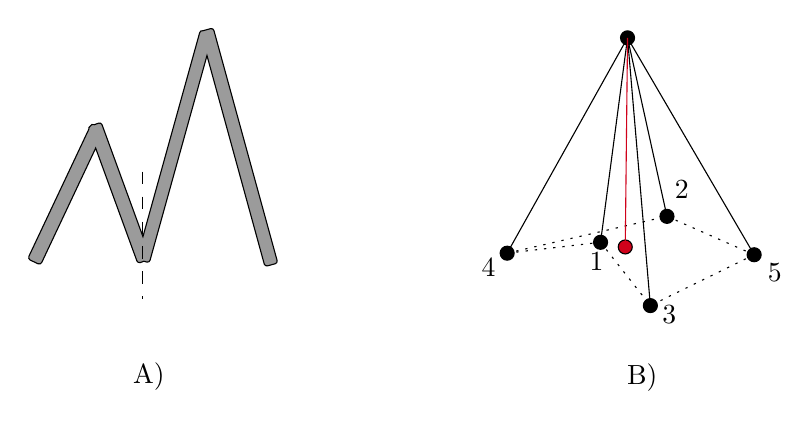
\begin{tikzpicture}[x=0.75pt,y=0.75pt,yscale=-1,xscale=1]
%uncomment if require: \path (0,300); %set diagram left start at 0, and has height of 300

%Shape: Circle [id:dp11222352082345399] 
\draw  [color={rgb, 255:red, 0; green, 0; blue, 0 }  ,draw opacity=1 ][fill={rgb, 255:red, 208; green, 2; blue, 27 }  ,fill opacity=1 ] (377.03,167.5) .. controls (377.03,165.64) and (378.54,164.13) .. (380.41,164.13) .. controls (382.27,164.13) and (383.78,165.64) .. (383.78,167.5) .. controls (383.78,169.36) and (382.27,170.88) .. (380.41,170.88) .. controls (378.54,170.88) and (377.03,169.36) .. (377.03,167.5) -- cycle ;
%Shape: Path Data [id:dp8182583139198897] 
\draw  [fill={rgb, 255:red, 155; green, 155; blue, 155 }  ,fill opacity=1 ] (93.08,172.01) -- (121.95,110.81) .. controls (121.81,110.21) and (122.1,109.59) .. (122.65,109.31) -- (122.7,109.22) .. controls (123.02,108.54) and (123.84,108.25) .. (124.52,108.57) -- (124.58,108.6) -- (126.61,107.86) .. controls (127.31,107.6) and (128.08,107.96) .. (128.34,108.66) -- (148.03,162.53) -- (175.37,64.22) .. controls (175.56,63.54) and (176.26,63.14) .. (176.93,63.33) -- (176.93,63.33) -- (180.65,62.31) .. controls (181.33,62.12) and (182.04,62.53) .. (182.22,63.21) -- (212.66,174.01) .. controls (212.85,174.7) and (212.45,175.4) .. (211.76,175.59) -- (208.05,176.61) .. controls (207.36,176.8) and (206.66,176.4) .. (206.47,175.71) -- (178.88,75.27) -- (151.45,173.9) .. controls (151.27,174.57) and (150.57,174.97) .. (149.89,174.78) -- (148.49,174.39) -- (146.83,175) .. controls (146.13,175.25) and (145.36,174.89) .. (145.1,174.19) -- (125.25,119.88) -- (99.29,174.93) .. controls (98.96,175.62) and (98.15,175.91) .. (97.46,175.59) -- (93.74,173.83) .. controls (93.06,173.51) and (92.76,172.69) .. (93.08,172.01) -- cycle ;
%Straight Lines [id:da03607049223761194] 
\draw  [dash pattern={on 4.5pt off 4.5pt}]  (148,131.25) -- (148,192.75) ;
%Straight Lines [id:da34790747177561565] 
\draw    (323.5,170.5) -- (381.5,66.75) ;
%Straight Lines [id:da09353312608269171] 
\draw    (368.5,165.25) -- (381.5,66.75) ;
%Straight Lines [id:da8094378775009878] 
\draw    (392.5,195.75) -- (381.5,66.75) ;
%Straight Lines [id:da9853129200676738] 
\draw    (400.5,152.75) -- (381.5,66.75) ;
%Straight Lines [id:da553621067401576] 
\draw    (442.5,171.25) -- (381.5,66.75) ;
%Shape: Circle [id:dp6210014442111269] 
\draw  [color={rgb, 255:red, 0; green, 0; blue, 0 }  ,draw opacity=1 ][fill={rgb, 255:red, 0; green, 0; blue, 0 }  ,fill opacity=1 ] (320.13,170.5) .. controls (320.13,168.64) and (321.64,167.13) .. (323.5,167.13) .. controls (325.36,167.13) and (326.88,168.64) .. (326.88,170.5) .. controls (326.88,172.36) and (325.36,173.88) .. (323.5,173.88) .. controls (321.64,173.88) and (320.13,172.36) .. (320.13,170.5) -- cycle ;
%Shape: Circle [id:dp07979906261849534] 
\draw  [color={rgb, 255:red, 0; green, 0; blue, 0 }  ,draw opacity=1 ][fill={rgb, 255:red, 0; green, 0; blue, 0 }  ,fill opacity=1 ] (389.13,195.75) .. controls (389.13,193.89) and (390.64,192.38) .. (392.5,192.38) .. controls (394.36,192.38) and (395.88,193.89) .. (395.88,195.75) .. controls (395.88,197.61) and (394.36,199.13) .. (392.5,199.13) .. controls (390.64,199.13) and (389.13,197.61) .. (389.13,195.75) -- cycle ;
%Shape: Circle [id:dp5673260807000834] 
\draw  [color={rgb, 255:red, 0; green, 0; blue, 0 }  ,draw opacity=1 ][fill={rgb, 255:red, 0; green, 0; blue, 0 }  ,fill opacity=1 ] (439.13,171.25) .. controls (439.13,169.39) and (440.64,167.88) .. (442.5,167.88) .. controls (444.36,167.88) and (445.88,169.39) .. (445.88,171.25) .. controls (445.88,173.11) and (444.36,174.63) .. (442.5,174.63) .. controls (440.64,174.63) and (439.13,173.11) .. (439.13,171.25) -- cycle ;
%Shape: Circle [id:dp9384795785708336] 
\draw  [color={rgb, 255:red, 0; green, 0; blue, 0 }  ,draw opacity=1 ][fill={rgb, 255:red, 0; green, 0; blue, 0 }  ,fill opacity=1 ] (365.13,165.25) .. controls (365.13,163.39) and (366.64,161.88) .. (368.5,161.88) .. controls (370.36,161.88) and (371.88,163.39) .. (371.88,165.25) .. controls (371.88,167.11) and (370.36,168.63) .. (368.5,168.63) .. controls (366.64,168.63) and (365.13,167.11) .. (365.13,165.25) -- cycle ;
%Shape: Circle [id:dp12037863567184737] 
\draw  [color={rgb, 255:red, 0; green, 0; blue, 0 }  ,draw opacity=1 ][fill={rgb, 255:red, 0; green, 0; blue, 0 }  ,fill opacity=1 ] (397.13,152.75) .. controls (397.13,150.89) and (398.64,149.38) .. (400.5,149.38) .. controls (402.36,149.38) and (403.88,150.89) .. (403.88,152.75) .. controls (403.88,154.61) and (402.36,156.13) .. (400.5,156.13) .. controls (398.64,156.13) and (397.13,154.61) .. (397.13,152.75) -- cycle ;
%Straight Lines [id:da22542851029214594] 
\draw  [dash pattern={on 0.84pt off 2.51pt}]  (323.5,170.5) -- (400.5,152.75) ;
%Straight Lines [id:da12485449512147406] 
\draw  [dash pattern={on 0.84pt off 2.51pt}]  (323.5,170.5) -- (368.5,165.25) ;
%Straight Lines [id:da7630944702055986] 
\draw  [dash pattern={on 0.84pt off 2.51pt}]  (368.5,165.25) -- (392.5,195.75) ;
%Straight Lines [id:da47805425202020513] 
\draw  [dash pattern={on 0.84pt off 2.51pt}]  (442.5,171.25) -- (392.5,195.75) ;
%Straight Lines [id:da9226618888425706] 
\draw  [dash pattern={on 0.84pt off 2.51pt}]  (442.5,171.25) -- (400.5,152.75) ;
%Shape: Circle [id:dp14148118645559526] 
\draw  [color={rgb, 255:red, 0; green, 0; blue, 0 }  ,draw opacity=1 ][fill={rgb, 255:red, 0; green, 0; blue, 0 }  ,fill opacity=1 ] (378.13,66.75) .. controls (378.13,64.89) and (379.64,63.38) .. (381.5,63.38) .. controls (383.36,63.38) and (384.88,64.89) .. (384.88,66.75) .. controls (384.88,68.61) and (383.36,70.13) .. (381.5,70.13) .. controls (379.64,70.13) and (378.13,68.61) .. (378.13,66.75) -- cycle ;
%Straight Lines [id:da3118870689790747] 
\draw [color={rgb, 255:red, 208; green, 2; blue, 27 }  ,draw opacity=1 ]   (381.5,66.75) -- (380.41,167.5) ;

% Text Node
\draw (362,169) node [anchor=north west][inner sep=0.75pt]   [align=left] {1};
% Text Node
\draw (403,134.5) node [anchor=north west][inner sep=0.75pt]   [align=left] {2};
% Text Node
\draw (397,194.5) node [anchor=north west][inner sep=0.75pt]   [align=left] {3};
% Text Node
\draw (310,172) node [anchor=north west][inner sep=0.75pt]   [align=left] {4};
% Text Node
\draw (447.88,174.25) node [anchor=north west][inner sep=0.75pt]   [align=left] {5};
% Text Node
\draw (142,222) node [anchor=north west][inner sep=0.75pt]   [align=left] {A)};
% Text Node
\draw (380,222.5) node [anchor=north west][inner sep=0.75pt]   [align=left] {B)};


\end{tikzpicture}

    \caption{A) Illustration of two adjacent triangles of different heights. B) Example of the order of printing the edges of a tetrahedron.}
    \label{fig:printing_tets}
\end{figure}

Before printing the tetrahedra, the base on which they will be printed must be printed. 
It will lie flat on the bed and will therefore be printed in a planar way. 
The base will always be a Delaunay triangulation of the points that compose the base. 
In order to optimise printing time, a depth-first search algorithm was used to obtain the longest paths that allow the base to be printed without repeating an edge. 
The longer the paths, the less time will be lost in repositioning the print head. 
Once the paths have been obtained, four layers will be printed with a layer height equivalent to half the diameter of the extruder. 
Printing four layers on the base will cause the position of the nodes to be different. 
Initially, the tetrahedra of the base have their base points at z = 0 \textit{mm}, but after printing the four layers, they must be moved to z = 0.8 \textit{mm} for an extruder with a diameter of 0.4 \textit{mm}. 
If this is not done, the extruder will pass through the four layers when printing the edges, breaking them.
This displacement must therefore be transmitted to all nodes of the structure. 
Then, all the print paths for all the edges are generated according to the order mentioned above.

\end{document}